\documentclass{minimal}
\usepackage{tikz}
\usetikzlibrary{patterns}

\begin{document}

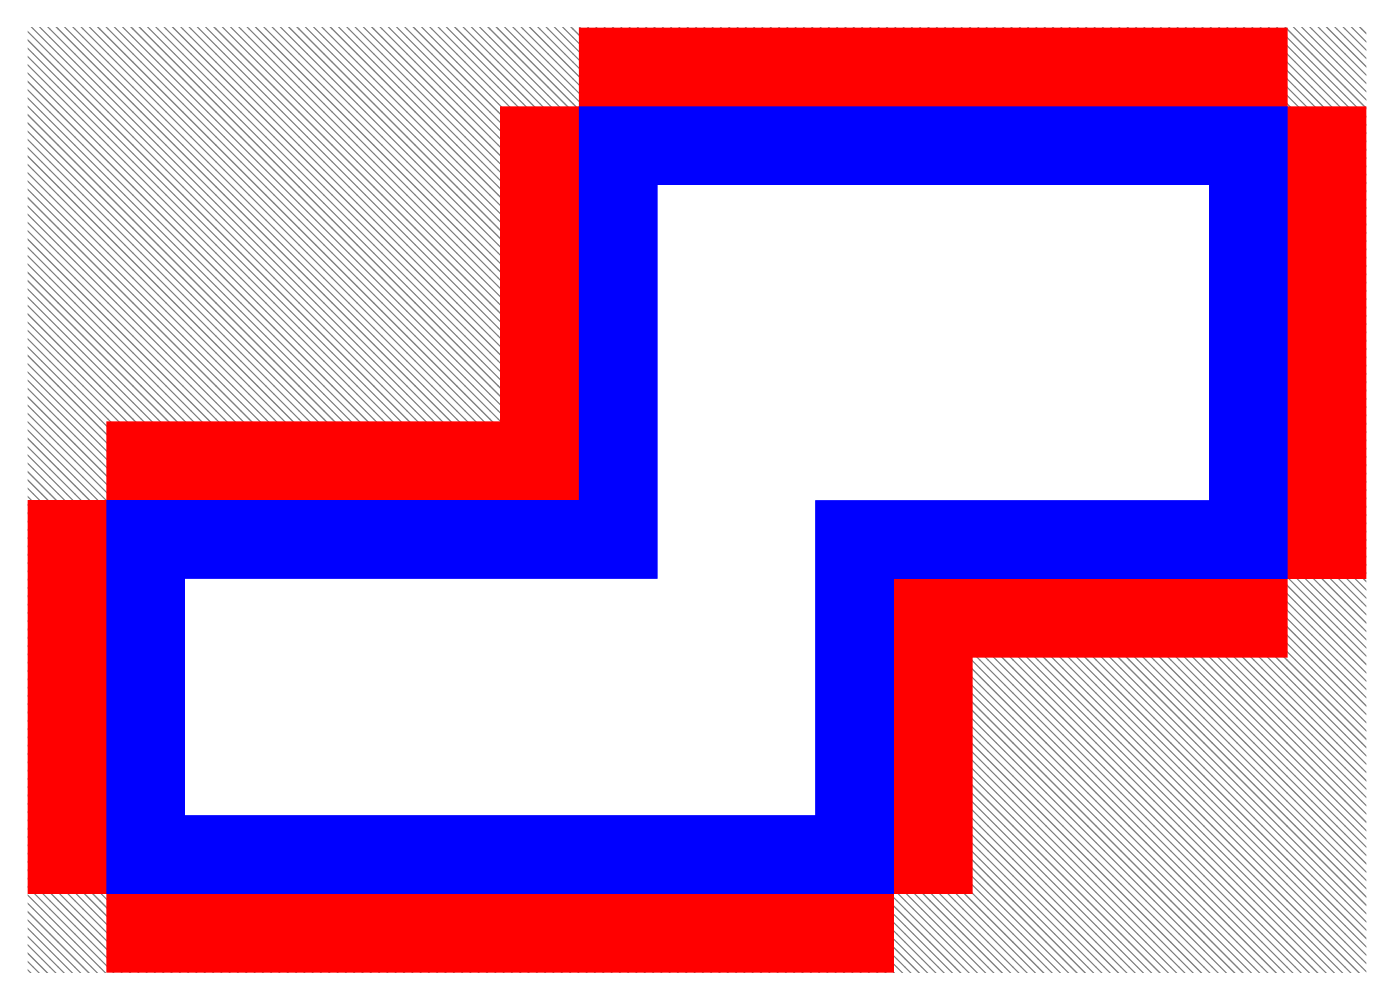
\begin{tikzpicture}[auto]
    \fill [pattern=north west lines, pattern color=gray] (-1, -1) rectangle (16, 11);
    \fill [red] (-1, 0) -- (-1, 5) -- (0, 5) -- (0, 6) -- (5, 6) -- (5, 10) -- (6, 10) -- (6, 11) -- (15, 11) --
                (15, 10) -- (16, 10) -- (16, 4) -- (15, 4) -- (15, 3) -- (11, 3) -- (11, 0) -- (10, 0) -- (10, -1) --
                (0, -1) -- (0, 0) -- cycle;
    \fill [blue] (0, 0) -- (10, 0) -- (10, 4) -- (15, 4) -- (15, 10) -- (6, 10) -- (6, 5) -- (0, 5) -- cycle;
    \fill [white] (1, 1) -- (9, 1) -- (9, 5) -- (14, 5) -- (14, 9) -- (7, 9) -- (7, 4) -- (1, 4) -- cycle;

\end{tikzpicture}

\end{document}
